\documentclass[11pt]{beamer}
\usetheme{Warsaw}
\usepackage[utf8]{inputenc}
\usepackage{amsmath}
\usepackage{amsfonts}
\usepackage{amssymb}
\usepackage{graphicx}
\author[Andrew Rosen]{Andrew Rosen \qquad Brendan Benshoof \qquad Robert W. Harrison \qquad Anu G. Bourgeois}
\title{MapReduce on a Chord Distributed Hash Table}
%\setbeamercovered{transparent} 
%\setbeamertemplate{navigation symbols}{} 
%\logo{} 
%\institute{} 
\date{} 
%\subject{} 
\begin{document}

\begin{frame}
\titlepage
\end{frame}

\begin{frame}
\tableofcontents
\end{frame}

\section{Introduction}

\subsection{Background}
\begin{frame}{Background}

\begin{itemize}
	\item Google's MapReduce \cite{mapreduce} paradigm is integral to data processing.
	\item Popular platforms for MapReduce, such as Hadoop \cite{hadoop}, are designed to be used in datacenters with a degree of centralization.  
	\item Until recently, analysis and optimization of MapReduce has largely remained constrained to that context.
\end{itemize}

\end{frame}

\subsection{Goals}
\begin{frame}{Goals}


\begin{itemize}
	\item We wanted build a more abstract system for MapReduce.
	\item We remove core assumptions \cite{hadoopAssumptions}:
	\begin{itemize}
		\item The system is centralized.
		\item Processing occurs in a static network.
	\end{itemize}
	\item The resulting system must be:
	\begin{itemize}
		\item Fault tolerant.
		\item Scalable.
		\item Completely decentralized.
	\end{itemize}
\end{itemize}

\end{frame}

\section{ChordReduce}


\begin{frame}{Features of ChordReduce}

ChordReduce is a decentralized framework for distributed computing:
\begin{itemize}
	\item Scalable.
	\item Load-Balancing.
	\item Decentralized:
	\begin{itemize}
		\item No centralized node is needed to maintain metadata.
		\item No central coordinator for tasks.
	\end{itemize}
	\item Fault tolerant:
	\begin{itemize}
		\item The loss of multiple nodes does not impact integrity.
		\item The network can withstand numerous simultaneous faults.
		\item Nodes in the network autonomously repair damage.
	\end{itemize}
	
\end{itemize}

\end{frame}



\subsection{System Architecture}
\begin{frame}{System Architecture}
ChordReduce has three layers
\begin{itemize}
	\item Chord \cite{Chord}, which handles routing and lookup.
	\item The Cooperative File System (CFS) \cite{CFS}, which handles storage and data replication.
	\item MapReduce.
\end{itemize}

\end{frame}

\subsection{Chord}

\begin{frame}{Chord}
Chord is a distributed hash table (DHT), where the nodes in the network are arranged in a ring overlay.
\begin{itemize}
	\item Nodes and files are assigned a $m$-bit key.
	\item Chord gives a high probability $\log_{2} N$ lookup time for any key.
	\item Nodes know their predecessors and successors in the ring.
	\item Nodes also maintain a table of $m$ shortcuts, called fingers.
	\item Nodes are responsible for files with keys between their predecessor's and theirs.
\end{itemize}


\end{frame}

\begin{frame}{A Chord Network}
\begin{figure}
    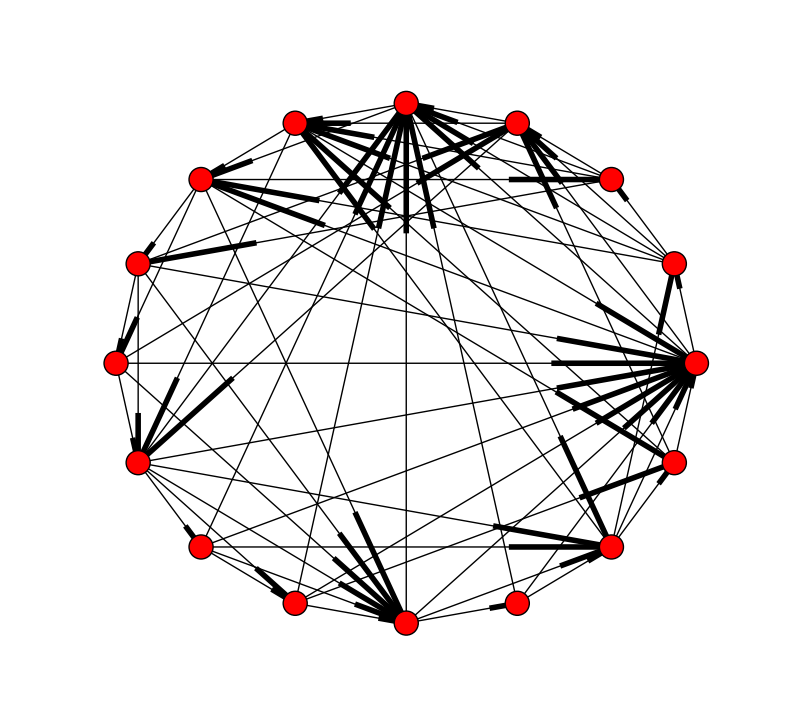
\includegraphics[width=0.6\linewidth]{chordreal}
    \caption{A Chord ring 16 nodes where $m=4$.}
    \label{chordreal}
\end{figure}
\end{frame}

\subsection{CFS}
\begin{frame}{CFS}
The Cooperative File System runs on top of Chord.

\begin{itemize}
	\item Files are split up, each block given a key based on their contents.
	\item Each block is stored according to their key.
	\item The hashing process guarantees that the keys are distributed near evenly among nodes.
	\item A keyfile is created and stored where the whole file would have been found.
	\item To retrieve a file, the node gets the keyfile and sends a request for each block listed in the keyfile.
\end{itemize}
\end{frame}
\begin{frame}{Fault Tolerance}

\begin{itemize}
	\item Each node maintains a list of its $s$ closest successors.
	\item Nodes back up data they're responsible for to their successors.
	\item When a node's predecessor fails, the node can immediately take over.
	\item The network will only lose data if $s+1$ successive nodes fail simultaneously.
	\item The chances of this are $r^{s+1}$, where $r$ is the failure rate.
\end{itemize}

\end{frame}






\subsection{MapReduce Module}

\begin{frame}{Starting a MapReduce Job}
\begin{itemize}
	\item Jobs can be started at an arbitrary node, denoted the \emph{stager}.
	\item The stager retrieves the keyfile and sends a map task for each key.
	\begin{itemize}
		\item This process can be streamlined recursively by bundling keys and sending them to the best finger.
		\item The resulting flow of data resembles a tree \cite{leemap}.
	\end{itemize}
	\item Once the stager has sent a map to every node, its job is done.
\end{itemize}
\end{frame}


\begin{frame}{Data Flow}
\begin{itemize}
	\item Results can be sent back via the overlay, or by initiating a direct connection.
	\item If a node receives multiple reduce results, they reduced into one before being sent along.
\end{itemize}
 
\end{frame}


\begin{frame}{Fault Tolerance of Map Jobs}
\begin{itemize}
	\item Each node backups their map tasks; removes it when the task is processed.
	\item If the immediate successor detects the node's failure, it takes over the task.
	\item If a node detects a new predecessor responsible for a key and map task pair in it's queue, it sends it to the predecessor.
	\item This allows node to further distribute the work during execution.
\end{itemize}
\end{frame}



\begin{frame}{Fault Tolerance of Reduces}
\begin{itemize}
	\item Individual reduces are backed up in a similar manner; if the original holder of the reduce fails before the reduce is sent, his successor sends his backup.
	\item Results are sent back to a key, rather than to a specific node.
	\item This ensures that if node receiving the data fails, his successor will take over.
\end{itemize}
\end{frame}



\section{Experiments}

\subsection{Experiments}
\begin{frame}{Experiment Goals}
We wanted to confirm that ChordReduce met our goals:

\begin{itemize}
    \item ChordReduce provides significant speedup during a distributed job.
    \item ChordReduce scales.
    \item ChordReduce handles churn during execution.
\end{itemize}

\end{frame}


\begin{frame}{Experiment Details}
Our initial test was a Monte Carlo approximation of $\pi$.

\begin{itemize}
	\item Map jobs were sent to randomly generated hash addresses.
	\begin{itemize}
		\item Map consisted of generating random coordinates from 0 to 1.
		\item ``Hits'' were defined as $x^{2} + y^{2} < 1^{2}$.
		\item The results were hits and total numbers generated.
	\end{itemize}
	\item Reducing the results was a matter of combining the two fields.
	\item The ratio of hits to generated results approximates $\frac{\pi}{4}$.
\end{itemize}

\end{frame}

\begin{frame}{Variables}
We ran the experiment using Amazon's Elastic Cloud Compute \cite{amazon-instances} and varied the following:
	\begin{itemize}
		\item Network size.
		\item Problem size.
		\item Rate of churn.
	\end{itemize}
\end{frame}


\subsection{Results}


\begin{frame}
\begin{figure}
    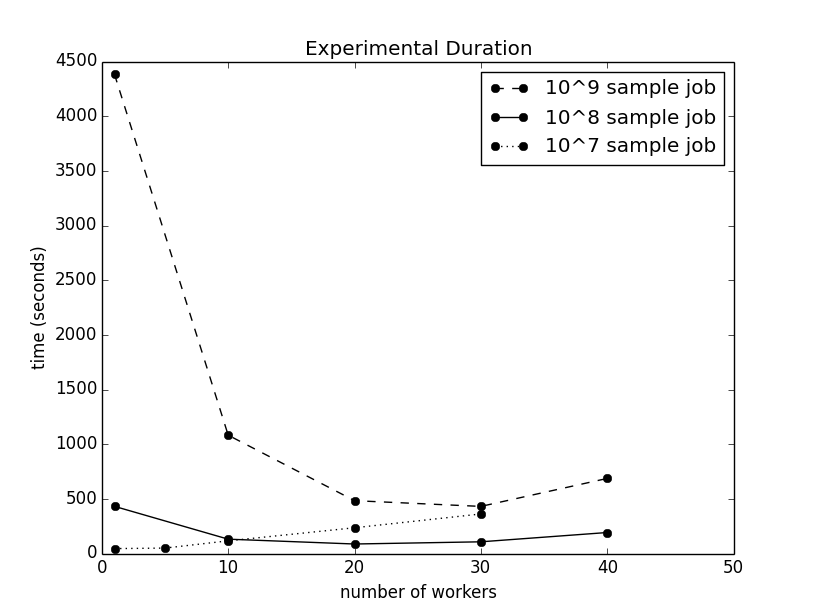
\includegraphics[width=0.65\linewidth]{expTime}
    \caption{For a sufficiently large job, it was almost always preferable to distribute it.  When the job is too small, such as with the $10^{7}$ data set, our runtime is dominated by the overhead.  Our results are what we would expect when overhead grows logarithmically to the number of workers.}
    \label{expTime}
\end{figure}

\end{frame}

\begin{frame}{Churn Results}
\begin{table}
    \centering
    \begin{tabular}{|r|r|r|} 
        \hline 
        Churn rate per second & Average runtime (s) & Speedup vs 0\% churn\\ \hline{}
        0.8\% & 191.25 & 2.15 \\ \hline
        0.4\% & 329.20 & 1.25 \\ \hline
        0.025\% & 431.86 & 0.95 \\ \hline 
        0.00775\%  & 445.47 & 0.92 \\ \hline 
        0.00250\% & 331.80  &  1.24 \\ \hline 
        0\% & 441.57 & 1.00 \\ \hline
    \end{tabular}
    \caption{The results of calculating $\pi$ by generating $10^8$ samples under churn. Churn is the chance for each node to join or leave the network. The large speedup is from joining nodes acquiring work during experimental runtime.} 
    \label{churnSpeed}
\end{table}

\end{frame}




\subsection{Conclusions}

\begin{frame}{Conclusions}
Our experiments established:
\begin{itemize}
	\item ChordReduce can operate under high rates of churn.
	\item Execution follows the desired logarithmic speedup.
	\item Speedup occurs on all problem sizes.
\end{itemize}

This makes ChordReduce an excellent platform for distributed and concurrent programming in cloud and loosely coupled environments.

\end{frame}


\begin{frame}{}
Questions?
\end{frame}

\bibliographystyle{IEEEtran}
\bibliography{CHRONUS}
\end{document}